\section{Description du robot d’accueil (UGV)}

\subsection{Choix du support d’accueil du drone d’inspection}

Pour accueillir le drone d’inspection, nous avions étudié la possibilité de réaliser une plateforme polyvalente embarquant les capteurs utiles (GNSS, boussole, IMU, etc.) et pouvant être placer sur n’importe véhicule mobile pouvant l’accueillir. Cette solution aurait l’avantage de proposer un décollage et un atterrissage du drone à la fois sur un navire comme un véhicule terrestre qu’ils soient fixes ou mobiles.
Cependant, pour des question de temps de travail dus à la réalisation matérielle et logicielle d’une telle plateforme combinée à celle du drone d’inspection, nous avons jugé bon de nous orienter vers un robot existant disposant d’une surface d'atterrissage suffisamment large et stable pour que l’UAV puisse s’y déposer.

Il nous a donc fallu étudier les différents supports mobiles disponibles à l’ENSTA Bretagne permettant d’embarquer une plateforme d'atterrissage. Le support mobile en question devait aussi être capable de se déplacer de manière stable pour faciliter l’accouplement avec le drone et devait être pilotable à distance ou capable de réaliser une trajectoire de manière autonome.

Pour compléter tous ces critères nous nous sommes orientés vers un robot déjà pris en main par le passé. Il s’agit du robot nommé Saturne, utilisé pour un précédent projet de recherche et cartographie magnétique d’un environnement plat, MagMap \cite{magmap}. Ce robot a été, en grande partie, fabriqué au sein de l’ENSTA Bretagne, sa conception et le matériel qu’il embarque sont connus et donc plus facile à maîtriser.

Ce robot à 4 roues se compose de deux parties indépendantes.
L’une contenant les éléments purement mécaniques du système tels que les moteurs, les contrôleurs de puissance, les batteries, les roues et une antenne radio pour réceptionner les commandes de pilotage à distance.
L’autre partie embarque les capteurs nécessaires à la navigation - un GNSS, une boussole, une IMU - et les équipements électroniques tel que l’ordinateur embarqué permettant de piloter le robot de façon autonome.

Caractéristiques techniques de Saturne :
\begin{itemize}
    \item 4 moteurs indépendants (4 $\times$ 500W)
    \item 3 batteries LiPo 6S (3h d’autonomie estimée)
    \item Télécommande radio (prioritaire)
    \item GNSS compatible RTK
    \item Cartes de commande Roboteq (avec mesure de tension et d’intensité) \cite{roboteq}
    \item PC embarqué Intel NUC (OS Ubuntu 18.04) \cite{nuc}
    \item LiDAR Velodyne Puck Lite \cite{velodyne}
    \item Caméra IP
\end{itemize}

Saturne est un robot de type char pouvant se déplacer dans un environnement plat de façon stable et à vitesse constante, soit les conditions adéquates pour l'atterrissage.

En plus de cela, Saturne est équipé d’une interface de contrôle ROS permettant de prendre contrôle de l’ensemble du système et cela de manière autonome afin de lui faire suivre une trajectoire prédéfinie. En cas de problème, il est toujours possible de reprendre la main sur le robot Saturne en actionnant la télécommande qui permet aussi de piloter les moteurs.
ROS a ainsi accès aux différentes mesures des capteurs propres au système et s’en sert pour commander le robot de manière autonome. Les données relatives au positionnement et au comportement dynamique de Saturne sont de cette façon consultables et peuvent être comparées avec celles du drone pour estimer la position relative, une information essentielle pour la manœuvre d’atterrissage.

\subsection{Plateforme d'atterrissage pour accouplement des deux robots}

Saturne est un robot initialement conçu pour tracter une charge au bout d’une corde comme son utilisation dans le projet MagMap. Il ne dispose donc pas de plateforme d’atterrissage pour accueillir le drone d’inspection. L’existence d’une telle surface d’accueil suffisamment large pour garantir la sûreté et la stabilité du drone lors des phases d’accouplement est essentielle pour la suite du projet.

\begin{figure}[H]
    \centering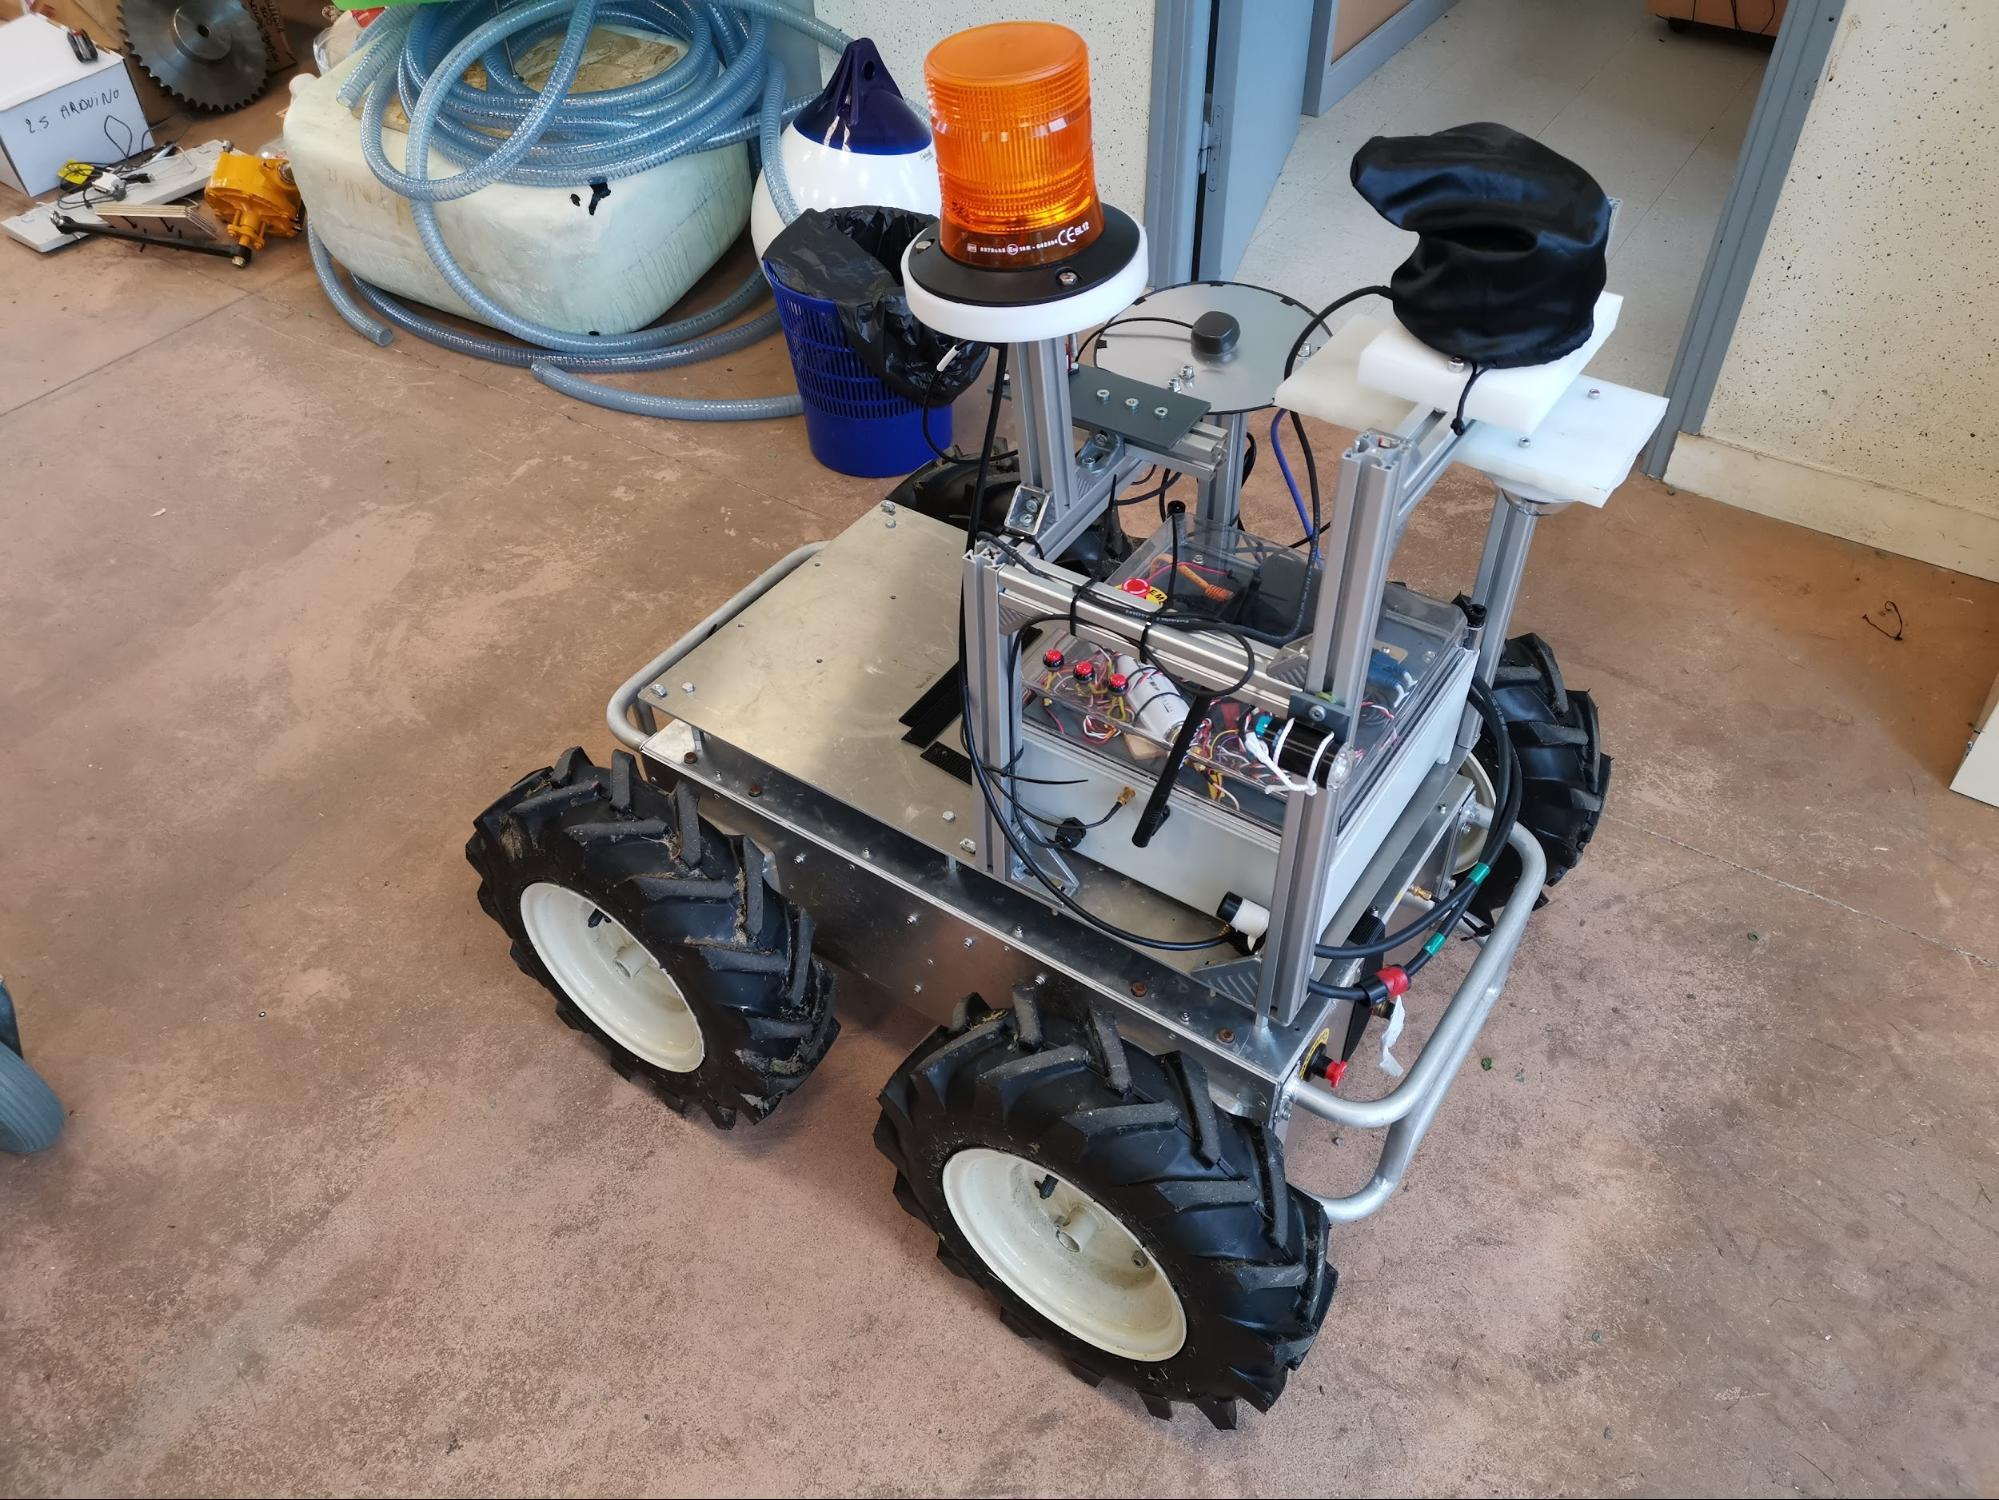
\includegraphics[width=150mm]{images/ugv/ugv1.jpg}
    \caption{Robot Saturne repris du projet MagMap \cite{magmap}}
\end{figure}

Nous avons donc dû concevoir une plateforme afin que Saturne puisse compléter son rôle de base d’appui. Etant donné sa fonction première nous avions d’abord pensé à lui faire tracter une remorque embarquant la plateforme d’atterrissage. Seulement pour des raisons pratiques, la mise en place d’une telle solution engendrerait une complexité de calcul supplémentaire du fait de l’articulation qui sépare la plateforme des capteurs utiles aux estimations des valeurs cinématiques.

La solution la plus adaptée au problème est donc de placer la plateforme directement sur le châssis de Saturne et le plus proche de son centre de gravité et de son axe de lacet afin de limiter les mouvements possibles causés par les rotations possibles du robot.

\begin{figure}[H]
    \centering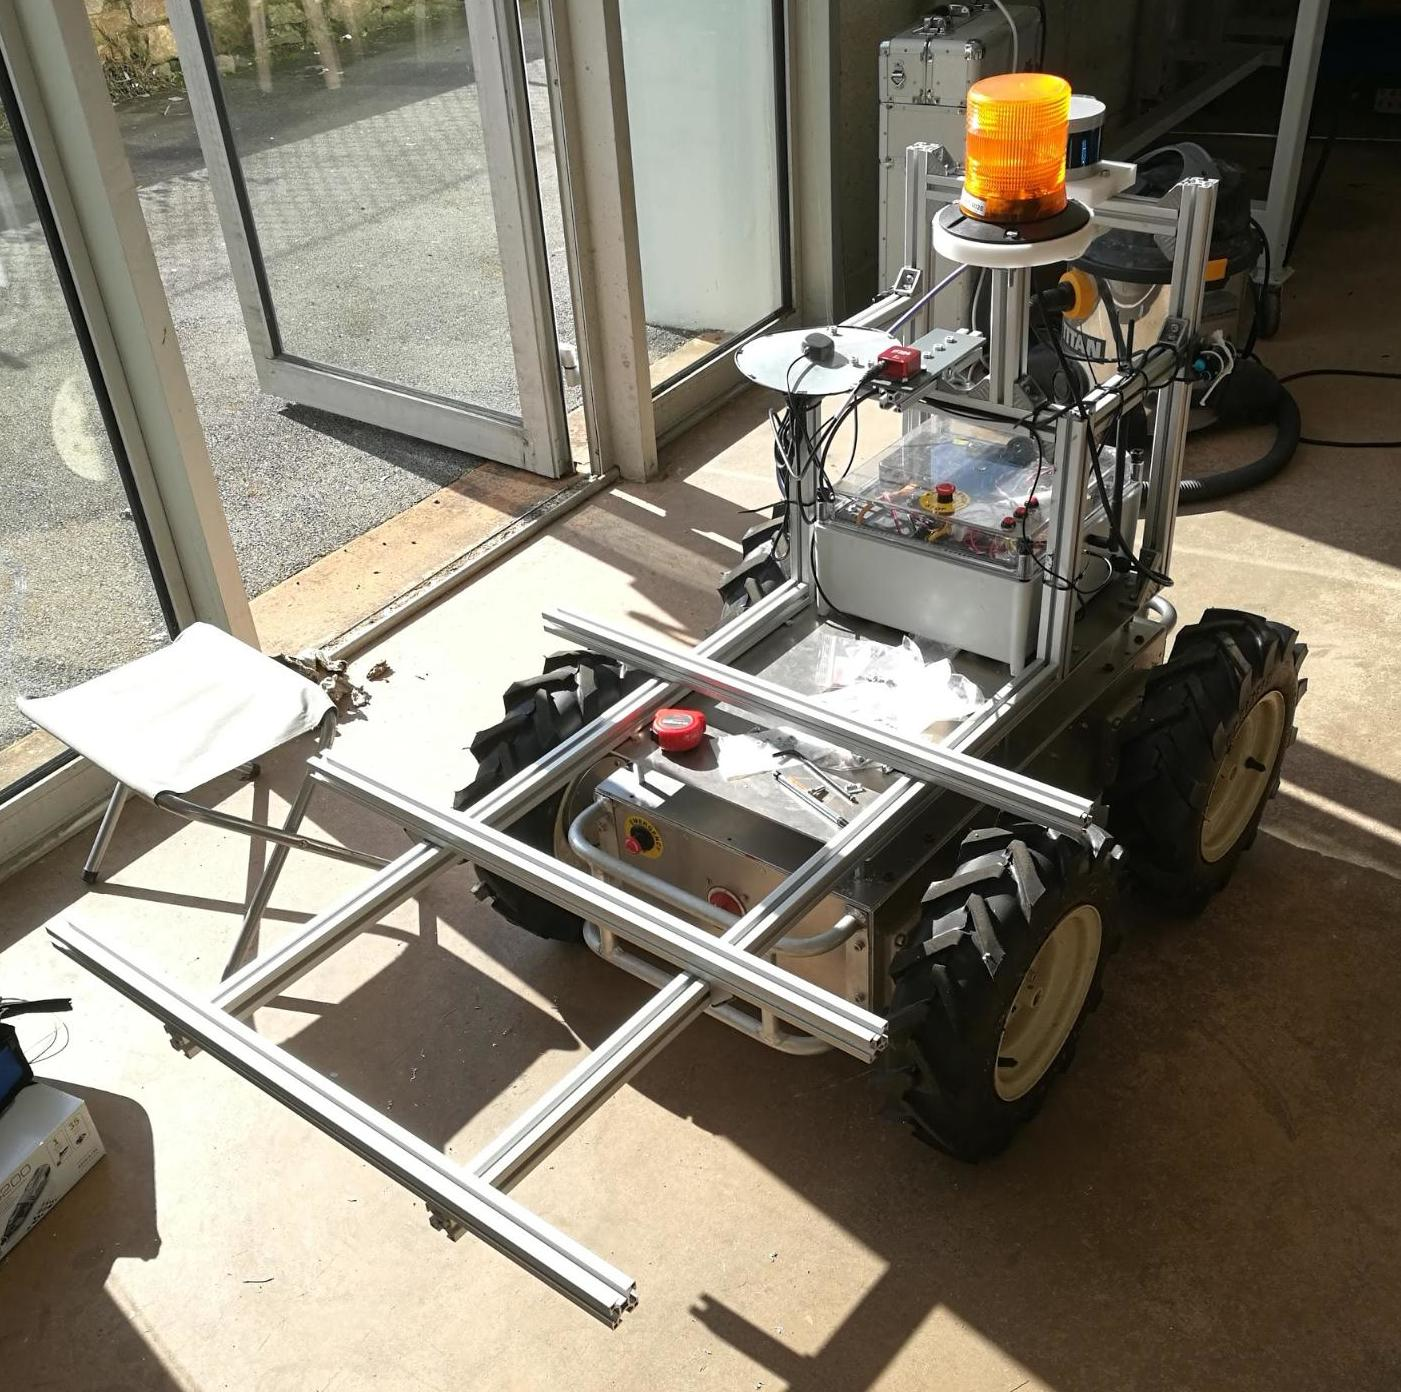
\includegraphics[width=150mm]{images/ugv/ugv2.jpg}
    \caption{Installation de la structure de la plateforme sur l'UGV Saturne}
\end{figure}

Aussi nous avons pris le soin de placer la plateforme à une certaine distance des équipements inamovibles de Saturne afin d’éviter au maximum tout conflit avec les hélices du de l’UAV.

\begin{figure}[H]
    \centering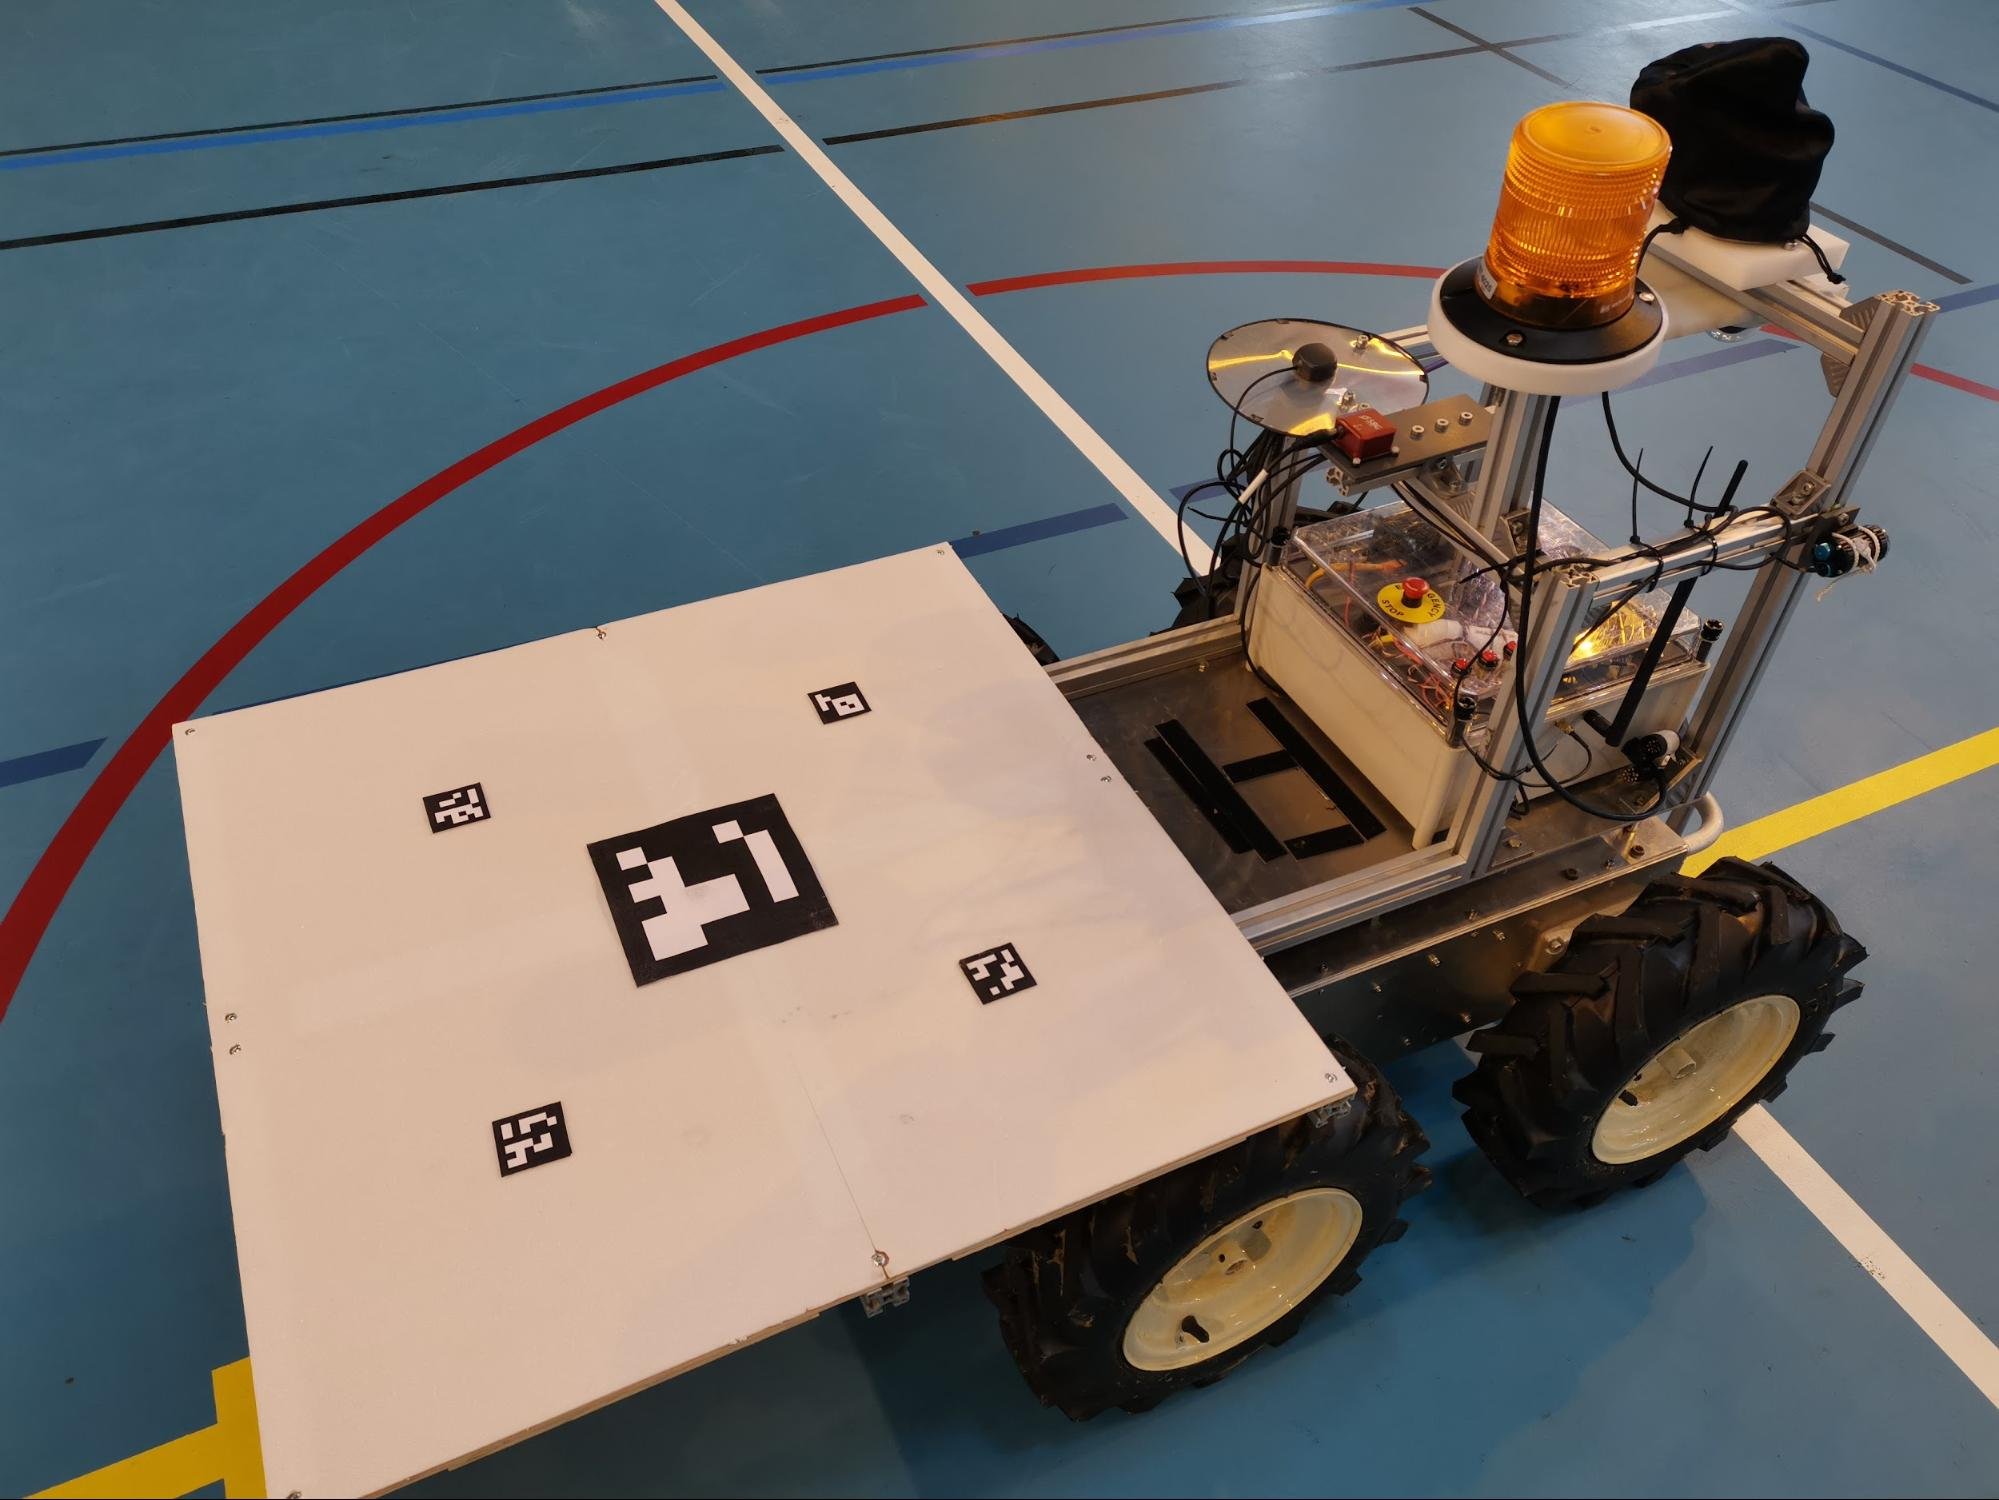
\includegraphics[width=150mm]{images/ugv/ugv3.jpg}
    \caption{UGV Saturne équipée de la plateforme d'accueil contenant les marqueurs ArUco}
\end{figure}

La plateforme prend ainsi la forme d’une extension à la structure initiale de Saturne. La surface en bois est de forme carrée et de dimension 750 $\times$ 750 mm. Sur cette surface est apposée un mousse semi-rigide de même dimension ayant pour but d’amortir le choc à l’atterrissage et de garantir une meilleure stabilité une fois le drone posé. La plateforme est excentrée de l’axe de lacet de Saturne d’une distance de 600 mm. Cette excentricité de la plateforme par rapport à l’UGV sera donc à prendre en compte dans les estimations de position relatives du drone par rapport à la surface d'atterrissage.

En notant $L$ l’excentricité de la plateforme on obtient la position du centre de la plateforme par la relation suivante :

\begin{align}
    \overrightarrow{P_{plateforme}} = L \times \begin{pmatrix}
    \cos(\theta) & -\sin(\theta) & 0 \\
    \sin(\theta) & \cos(\theta) & 0 \\
    0 & 0 & 1
    \end{pmatrix}
    \times \overrightarrow{P_{saturne}}
\end{align}

avec $\overrightarrow{P_{plateforme}}$ le vecteur position du centre de la plateforme et $\overrightarrow{P_{saturne}}$ le vecteur position du centre de Saturne.

\section{Navigation et commande de l’UGV Saturne}

\subsection{Architecture ROS}

\begin{figure}[H]
    \centering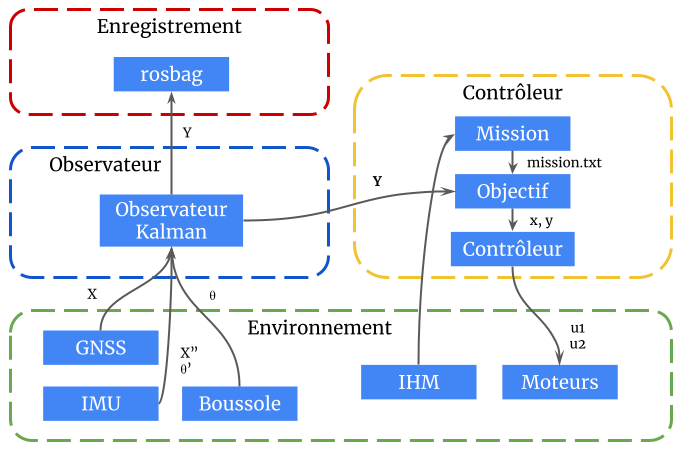
\includegraphics[width=150mm]{images/ugv/arch_ros.png}
    \caption{Architecture ROS}
\end{figure}

\begin{itemize}
    \item \textbf{Estimateur :}
    Ce nœud calcule une estimation de la position du robot. Il reçoit une estimation de la position du robot par le GNSS et les données de l’IMU. Entre chaque nouvelle mesure GNSS, il intègre la mesure donnée par l’IMU afin d’obtenir une fréquence plus élevée que le GNSS seul.
    \\
    \item \textbf{Mission :}
    Ce nœud gère les objectifs de la mission. C’est ce nœud qui lit le fichier texte contenant les objectifs et qui gère les conditions de fin d’objectif et de fin de mission.
    \\
    \item \textbf{Objectif :}
    Ce nœud calcule une commande en cap pour que le robot réalise son objectif courant. Le cap est calculé en utilisant la méthode des champs de potentiels.
    \\
    \item \textbf{Contrôleur :}
    Ce nœud prend le cap consigne et le convertit en commande à envoyer aux cartes de contrôle des moteurs.
    \\
    \item \textbf{IHM :}
    Une IHM a été développée afin de surveiller le déroulement de la mission. On y affiche les objectifs et la position estimée du robot en temps réel afin de vérifier que tout fonctionne correctement.
\end{itemize}